\documentclass[twocolumn]{article} % Two-column document

% Packages for formatting
\usepackage[utf8]{inputenc}
\usepackage{amsmath}
\usepackage{geometry}
\usepackage{graphicx}
\usepackage{lipsum} % for filler text
\usepackage{authblk} % For author affiliations
\usepackage[utf8]{inputenc}
\usepackage{hyperref}

\usepackage{textcomp}
\usepackage{charter}
\usepackage{framed}

\usepackage{verbatim}

\hypersetup{
    colorlinks=true,
    linkcolor=blue,
    filecolor=magenta,      
    urlcolor=cyan,
    pdftitle={Overleaf Example},
    pdfpagemode=FullScreen,
}

% Page setup
\geometry{a4paper, margin=0.5in}

% Title and Author formatting
\makeatletter
\renewcommand{\maketitle}{
    \bgroup\setlength{\parindent}{0pt}
        \begin{flushleft}
        \textbf{\@title\newline}
        
        \@author
        \end{flushleft}
    \egroup
}
\makeatother

% Title
\title{\fontsize{40}{1}\usefont{T1}{cmr}{b}{n} Modeling Student Performance: Using Multiple Linear Regression to Predict Exam Scores \vspace{0.05cm}}

% Authors
\author[1]{Victoria Blante}
\author[2]{Chelyah Miller}
\author[3]{Xiaonan Song}
\author[4]{Emma Juan Salazar}

% Author affiliations
\affil[*]{University of San Francisco, Master of Science in Data Science\newline}

% Email
\affil[1]{vbblante@dons.usfca.edu}
\affil[2]{cmiller9@dons.usfca.edu}
\affil[3]{xsong20@dons.usfca.edu}
\affil[4]{ejuansalazar@dons.usfca.edu}

\renewcommand\Authands{ and }

\date{\today} % You can manually enter a date if needed

% Define path where images are stored
\graphicspath{ {./images/} }

% Define abstract format
\renewenvironment{abstract}
 {\small
  \begin{center}
  \bfseries \abstractname\vspace{-.5em}\vspace{0pt}
  \end{center}
  \list{}{%
    \setlength{\leftmargin}{10mm}% <---------- Change margin here
    \setlength{\rightmargin}{\leftmargin}%
  }%
  \item\relax}
 {\endlist}

% Begin the document
\begin{document}

% Print out title and abstract
\twocolumn[
\begin{@twocolumnfalse}

\maketitle

\begin{abstract}
\textit{
    \lipsum[1]
    \bigskip}
\end{abstract}

% Keywords
\textbf{Keywords:} Multiple Linear Regression, Modeling

All of the scripts and data for this project can be found on our \href{https://github.com/cztm/linear-regression}{Git Repository}.
\newline\newline\newline
\end{@twocolumnfalse}
]

% INTRODUCTION
\section{Introduction}
\subsection*{Our Dataset}
Our selected dataset is \href{https://www.kaggle.com/datasets/lainguyn123/student-performance-factors}{Student Performance Factors}.

The ``Student Performance Factors'' dataset contains 19 variables that
may influence students' exam scores. It is designed to help researchers
analyze the potential impact of these factors on student performance.
The dataset includes information such as study time
(\texttt{Hours\_Studied}), attendance (\texttt{Attendance}), parental
involvement (\texttt{Parental\_Involvement}), access to resources
(\texttt{Access\_to\_Resources}), and participation in extracurricular
activities (\texttt{Extracurricular\_Activities}). Additionally, it
covers socioeconomic and background data such as family income
(\texttt{Family\_Income}), motivation level
(\texttt{Motivation\_Level}), tutoring sessions
(\texttt{Tutoring\_Sessions}), school type (\texttt{School\_Type}),
sleep hours (\texttt{Sleep\_Hours}), and parental education level
(\texttt{Parental\_Education\_Level}).

\subsection*{Purpose and Applications}\label{purpose-and-applications}

Researchers can use this dataset to build regression models for
predicting exam scores (\texttt{Exam\_Score}) and to identify
significant factors affecting student academic performance. The
dataset's potential applications include:

\begin{itemize}
\item
    Supporting educational decision-making
\item
    Assisting in policy formulation
\item
    Optimizing the allocation of educational resources
\end{itemize}

Ultimately, the goal is to better understand and improve the key factors
influencing student success, thereby enabling educators and policymakers
to provide more targeted support.

\subsection*{Variable Descriptions}\label{variable-descriptions}

\begin{itemize}
\item
  \texttt{Hours\_Studied}: Daily study hours.
\item
  \texttt{Attendance}: Attendance rate (percentage).
\item
  \texttt{Parental\_Involvement}: Parent involvement (Low, Medium, High).
\item
  \texttt{Access\_to\_Resources}: Resource accessibility (Low, Medium, High).
\item
  \texttt{Extracurricular\_Activities}: Participation in extracurricular
  activities.
\item
  \texttt{Sleep\_Hours}: Daily sleep hours.
\item
  \texttt{Previous\_Scores}: Prior exam scores.
\item
  \texttt{Motivation\_Level}: Motivation level (Low, Medium, High).
\item
  \texttt{Internet\_Access}: Internet access.
\item
  \texttt{Tutoring\_Sessions}: Number of tutoring sessions.
\item
  \texttt{Family\_Income}: Family income level (Low, Medium, High).
\item
  \texttt{Teacher\_Quality}: Teacher quality (Low, Medium, High).
\item
  \texttt{School\_Type}: School type (Public or Private).
\item
  \texttt{Peer\_Influence}: Peer influence (Positive, Neutral,
  Negative).
\item
  \texttt{Physical\_Activity}: Weekly physical activity hours.
\item
  \texttt{Learning\_Disabilities}: Presence of learning disabilities.
\item
  \texttt{Parental\_Education\_Level}: Parents' education level (High School, College, Postgraduate).
\item
  \texttt{Distance\_from\_Home}: Distance from home to school (Near, Moderate, Far).
\item
  \texttt{Gender}: Student gender (Male or Female).
\item
  \texttt{Exam\_Score}: Academic performance indicator (exam score).
\end{itemize}

% \cite{sample_reference}.

% METHODS
\section{Methods}
We used various methods to perform our analysis, from EDA all the way to Model Evaluation. Here's a detailed description of the methods and tools we used.

\begin{itemize}
\item
  \textbf{Exploratory Data Analysis}:
  Initial analysis includes
  correlation calculations to understand the relationships between
  predictors and exam scores.
\item
  \textbf{Multiple Linear Regression}:
  Regression models are built using
  significant predictors such as attendance, hours studied, and previous
  scores. The model is validated using metrics like adjusted R-squared,
  p-values, and F-statistics.
\item
  \textbf{ANOVA (Types I, II, and III)}:
  Variance analysis is conducted
  to understand the contribution of each predictor to the total variance
  in exam scores.
\item
  \textbf{Model Evaluation}:
  The model's prediction capability is
  visualized through plots of actual vs.~predicted exam scores,
  residuals distribution, and summary statistics.
\end{itemize}

% RESEARCH QUESTIONS

\section{Exploratory Data Analysis}
The Student Performance Factors dataset has 20 variables and 6607 observations. We have 7 numerical variables, including hours studied, attendance, sleep hours, previous scores, tutoring sessions, physical activity and exam score. The other 13 variables are categorical, having either 2 or 3 categories each.
This gives us enough room to be able to perform a comprehensive Multiple Linear Regression Analysis.

Before delving into our dataset, we checked for missing data. Only three of our columns had missing values (\texttt{Teacher\_Quality}, \texttt{Parental\_Education\_Level} and \texttt{Distance\_from\_Home}). Each of these columns has less than 2\% of missingness. Seeing as we have a substantial number of observations, we decided to go ahead and drop all observations with missing data (229 rows).

Our dataset size after this was of 20 variables and 6378 records.

\subsection*{Categorical variables}

Our first approach to get a sense of our categorical data was to plot the frequency for each category. See these plots in Supplementary Figure \ref{1:barplots}.

These plots allowed us to see that some categorical variables had similar shaped barplots. To optimize our categorical variables we drew up confusion tables to ascertain wether or not to collapse some of these variables.

We made confusion tables to check \texttt{Parental\_Involvment} against \texttt{Access\_to\_Resources} (Supplementary Table \ref{tab:confusion1}), \texttt{Family\_Income} against \texttt{Peer\_Influence} (Supplementary Table \ref{tab:confusion2}), \texttt{Distance\_from\_Home} against \texttt{Motivation\_Level} (Supplementary Table \ref{tab:confusion3}) and \texttt{Distance\_from\_Home} against \texttt{Motivation\_Level} (Supplementary Table \ref{tab:confusion3})

These confusion tables aided us to make the decision to drop the variables \texttt{Distance\_from\_Home}, \texttt{Peer\_Influence} and \texttt{Parental\_Involvment}.

\subsection*{Numerical Variables}

As a first approach, for the numerical variables, we drew boxplots to check their distributions and wether or not we see any outliers (Supplementary Figure \ref{2:boxplots})

From these boxplots, we saw that for tutoring sessions we have a few outliers in the upper levels but most of the observations are clustered around 1/2 tutoring sessions. We can also see that for exam score, most of the students in our dataset have scores clustered around 65 out of 100, and we have a few high performing students. We'll have to keep these in mind when picking our response variable.

Next, we decided to make a pairwise plot (Supplementary Figure \ref{3:pairwise}), a very powerful tool to try and get a first glance at which numerical variables seem to have linear relationships between one another.

A lot of our variables numerical variables are discreet and therefore the scatterplots show very distinct levels. Aside from these, there's a few scatterplots where we can see some sort of linearity between two variables. We can very clearly see that all of these plots include the variable \texttt{Exam\_Score}.

Looking at the histogram for Exam Score inside of the pairwise plot, we can very clearly see how it's clustered around lower scores, therefore indicating we don't have a normal distribution for these. We'll have to keep this fact in mind when analyzing this variable.

Lastly, we made a correlation heatmap (Figure \ref{4:corr-heatmap}), to assess how are variables are correlated between one another and get a first glance towards multicollinearity.

\begin{figure*}[h]
  \centering
  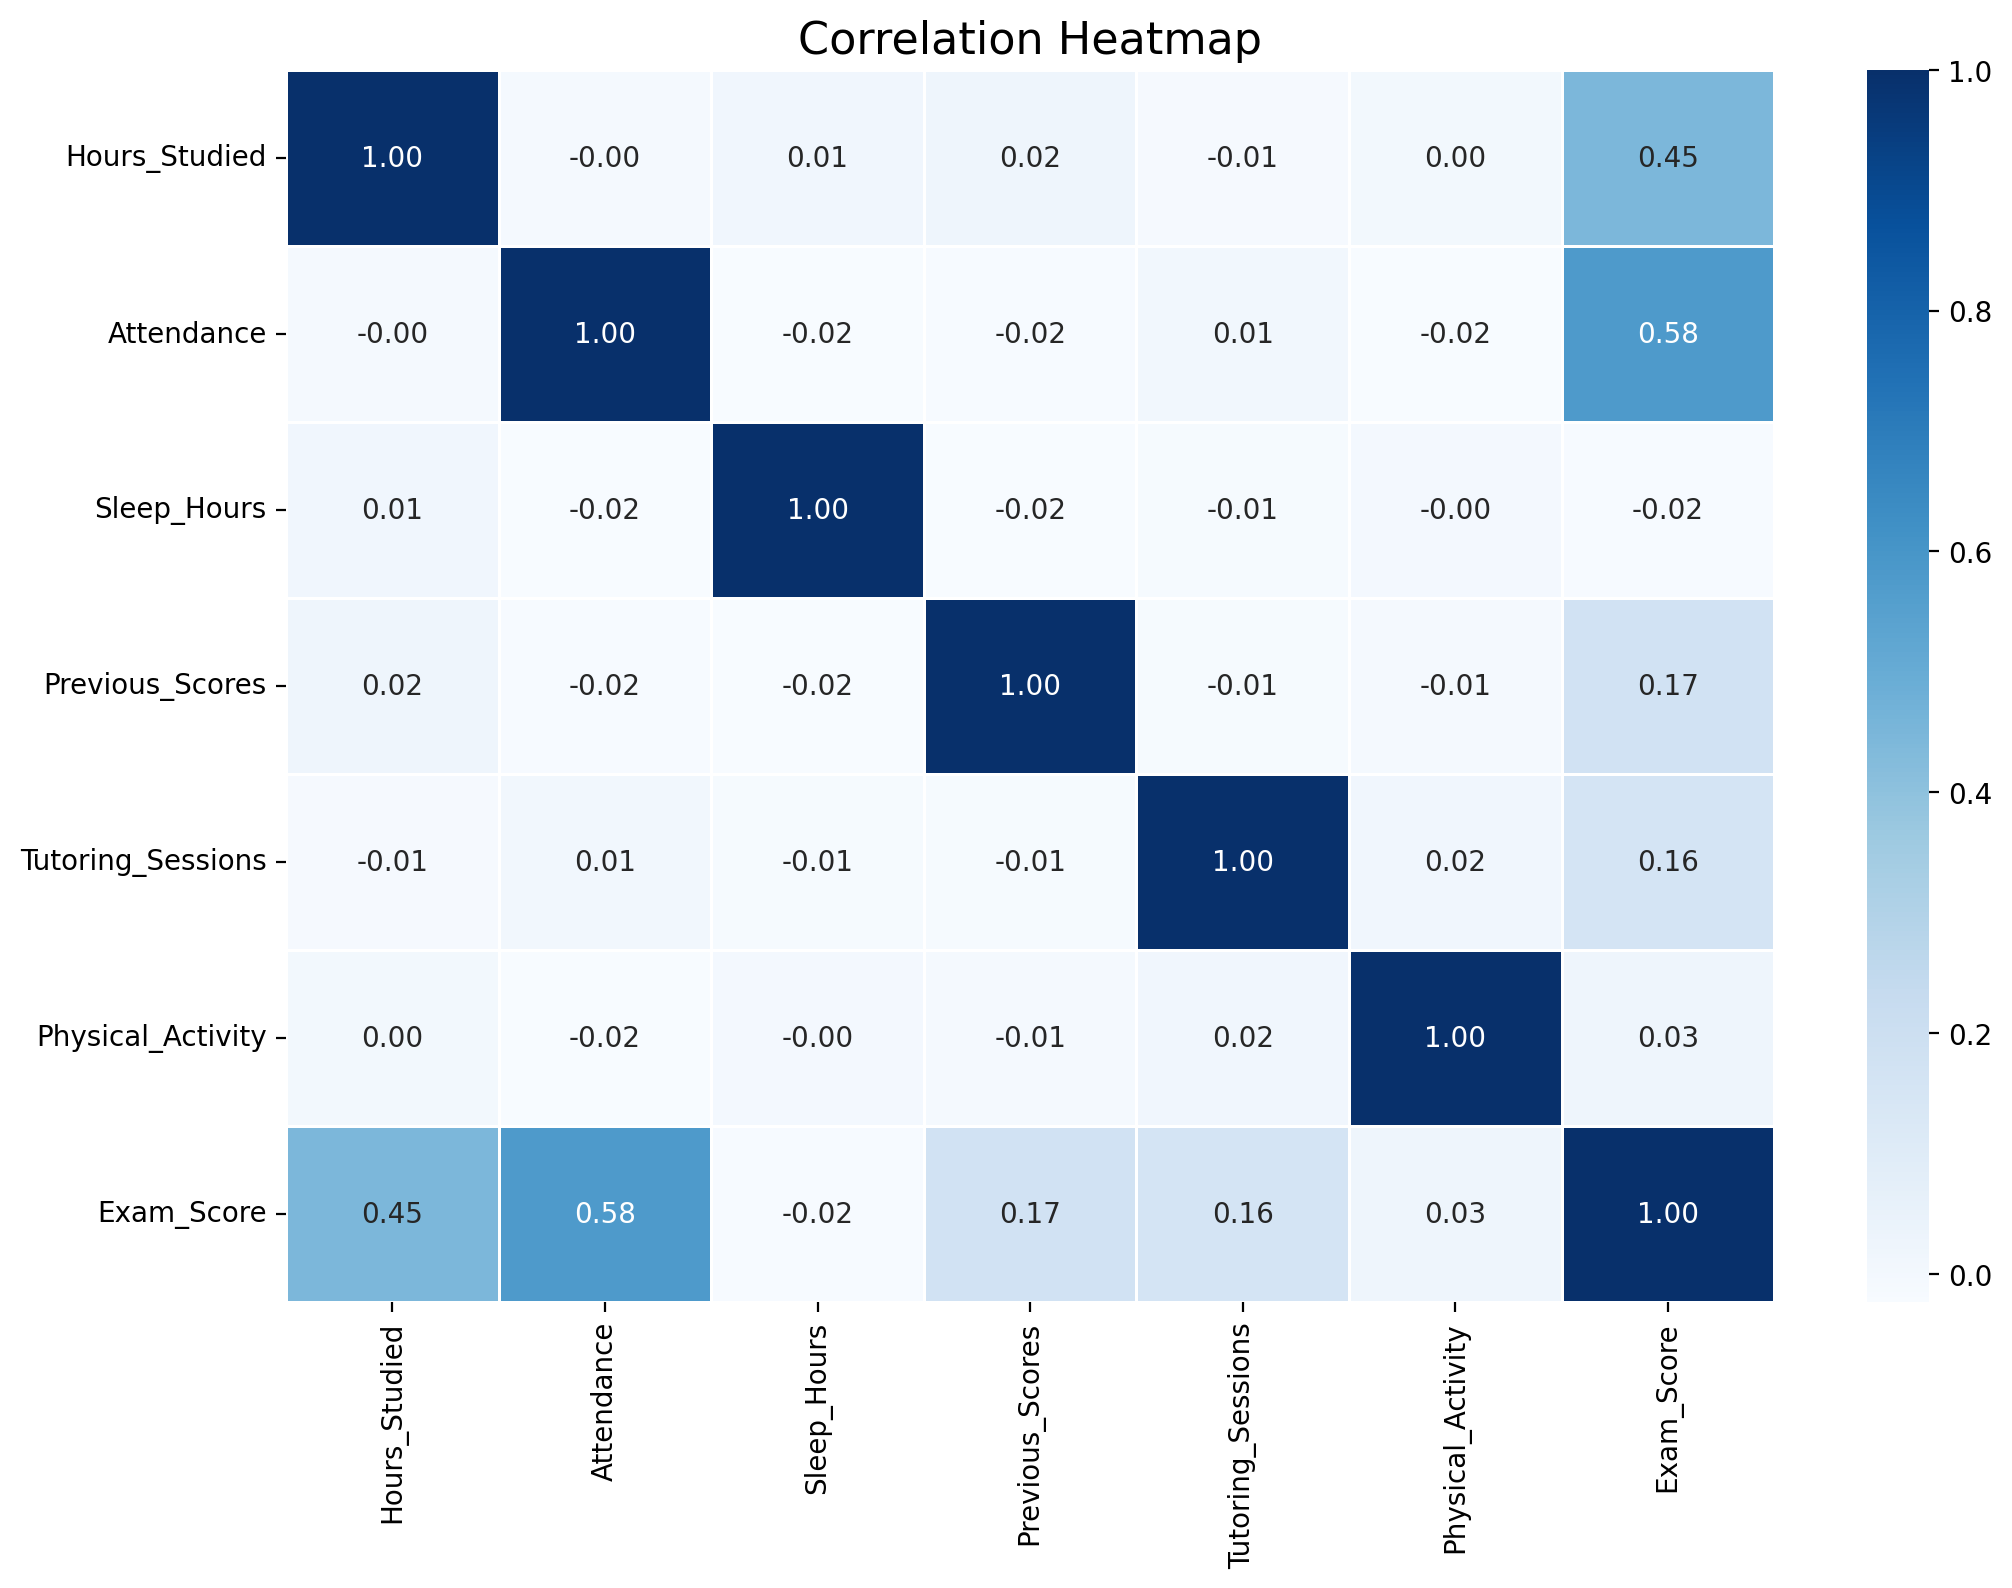
\includegraphics[width=1.3\columnwidth]{4-correlation-heatmap.png}
  \caption{Heatmap depicting the correlation between our numerical variables.}
  \label{4:corr-heatmap}
\end{figure*}

We can see how the variable that has the most correlation to other variables is Exam Score, and how there's next to no correlation among the other variables. This indicates that picking Exam Score as our response variable seems a prudent choice, as it looks to be correlated to our other variables and also makes it so we have lower chances of having multicollinearity.

\newpage
\section{Hypotheses}

\subsection*{Hypothesising based on our EDA}
Since we were able to see some linear relationship between a few of our numerical variables and \texttt{Exam\_Score}, we have decided to pick this variable as our response variable.

The correlation heatmap also supports our choice of response variable, where we can see correlation between exam scores and the rest of the variables.

In the context of our problem, modeling student performance, we think choosing exam scores as our response variable is a good way to ascertain how students perform, and which factors influence the way they score in tests.

We have initially seen linearity in the scatterplots between exam score and hours studied, attendance, previous scores and tutoring sessions. We'll try to assess wether or not these numerical variables are statistically significant when predicting exam scores.

In regards to our remaining categorical variables after discarding based on confusion tables, we'll check for significance for all of them and try to ascertain which variables are best to include in our model with the goal of predicting exam scores.

As previously stated, the correlation heatmap seems to indicate we don't have severe multicollinearity. Further checks need to be done to ensure this.

We have to consider the fact that Exam Scores are clustered around 65 out of 100, and we have what we could consider some outliers in the higher ranges. Based on this, we think we may encounter that the high scores have a different relationship to the predictors compared to the majority of the other scores, which are around the 65\%.

\subsection*{Research Questions}

Our main research question is the following:
\begin{itemize}
  \item
\textbf{Which factors are the most significant predictors of students' exam scores?}
\end{itemize}

We also have specific questions about our different variables and their impact on the student's performance.
\newline\newline
Regarding our numerical variables:
\begin{itemize}
\item
      \textbf{What is the combined effect of study habits, attendance, previous scores and tutoring sessions on exam outcomes?}
\end{itemize}
Regarding our categorical variables:
\begin{itemize}
\item
    \textbf{How do socioeconomic factors like access to resources or family income impact student performance?}
\item
    \textbf{Do other student habits like extracurricular activities, motivation level or internet access have an important effect on the student performance?}
\item
    \textbf{Does the hours a student spends doing physical activity impact their performance in tests?}
\item
    \textbf{Does wether or not a student have a learning disability systematically impact their exam performance?}
\item
    \textbf{Does the level of education of their parents indicate the performance of a student in exams?}
\item
    \textbf{Does school type or teacher quality significantly influence exam scores?}
\end{itemize}


\section{Multiple Regression Analysis}

\subsection*{Initial Model}
Our first approach to ascertain which predictors to include in our MLR model was to make a Simple Linear Regression model for each of our predictors. We compared metrics for each of these models, like $R^2$, and picked the highest performing size 1 models to make an initial MLR model %(Supplementary Table \ref{tab:intial-model})

\subsection*{Box-Cox Transformation}
\lipsum[1]
\subsection*{Splitting the Data Into Two Models}
\lipsum[1]

% RESULTS
\section{Results}
\subsection*{Low Scores Model}
\lipsum[1]
\subsection*{High Scores Model}
\lipsum[1]

% DISCUSSION
\section{Discussion}
\lipsum[1]

% CONCLUSION
\section{Conclusion}
\lipsum[1]

% References
% \begin{thebibliography}{99}
%     \bibitem{sample_reference}
%     Author Name, \textit{Title of the Reference}, Journal Name, VolumeIssue, Pages, Year.
    
%     \bibitem{example2}
%     Another Author, \textit{Another Paper}, Conference Name, Pages, Year.
% \end{thebibliography}

\newpage
\onecolumn

\section*{Supplementary Materials}

\renewcommand{\figurename}{Supplementary Figure}
\setcounter{figure}{0}

\begin{figure*}[h]
  \centering
  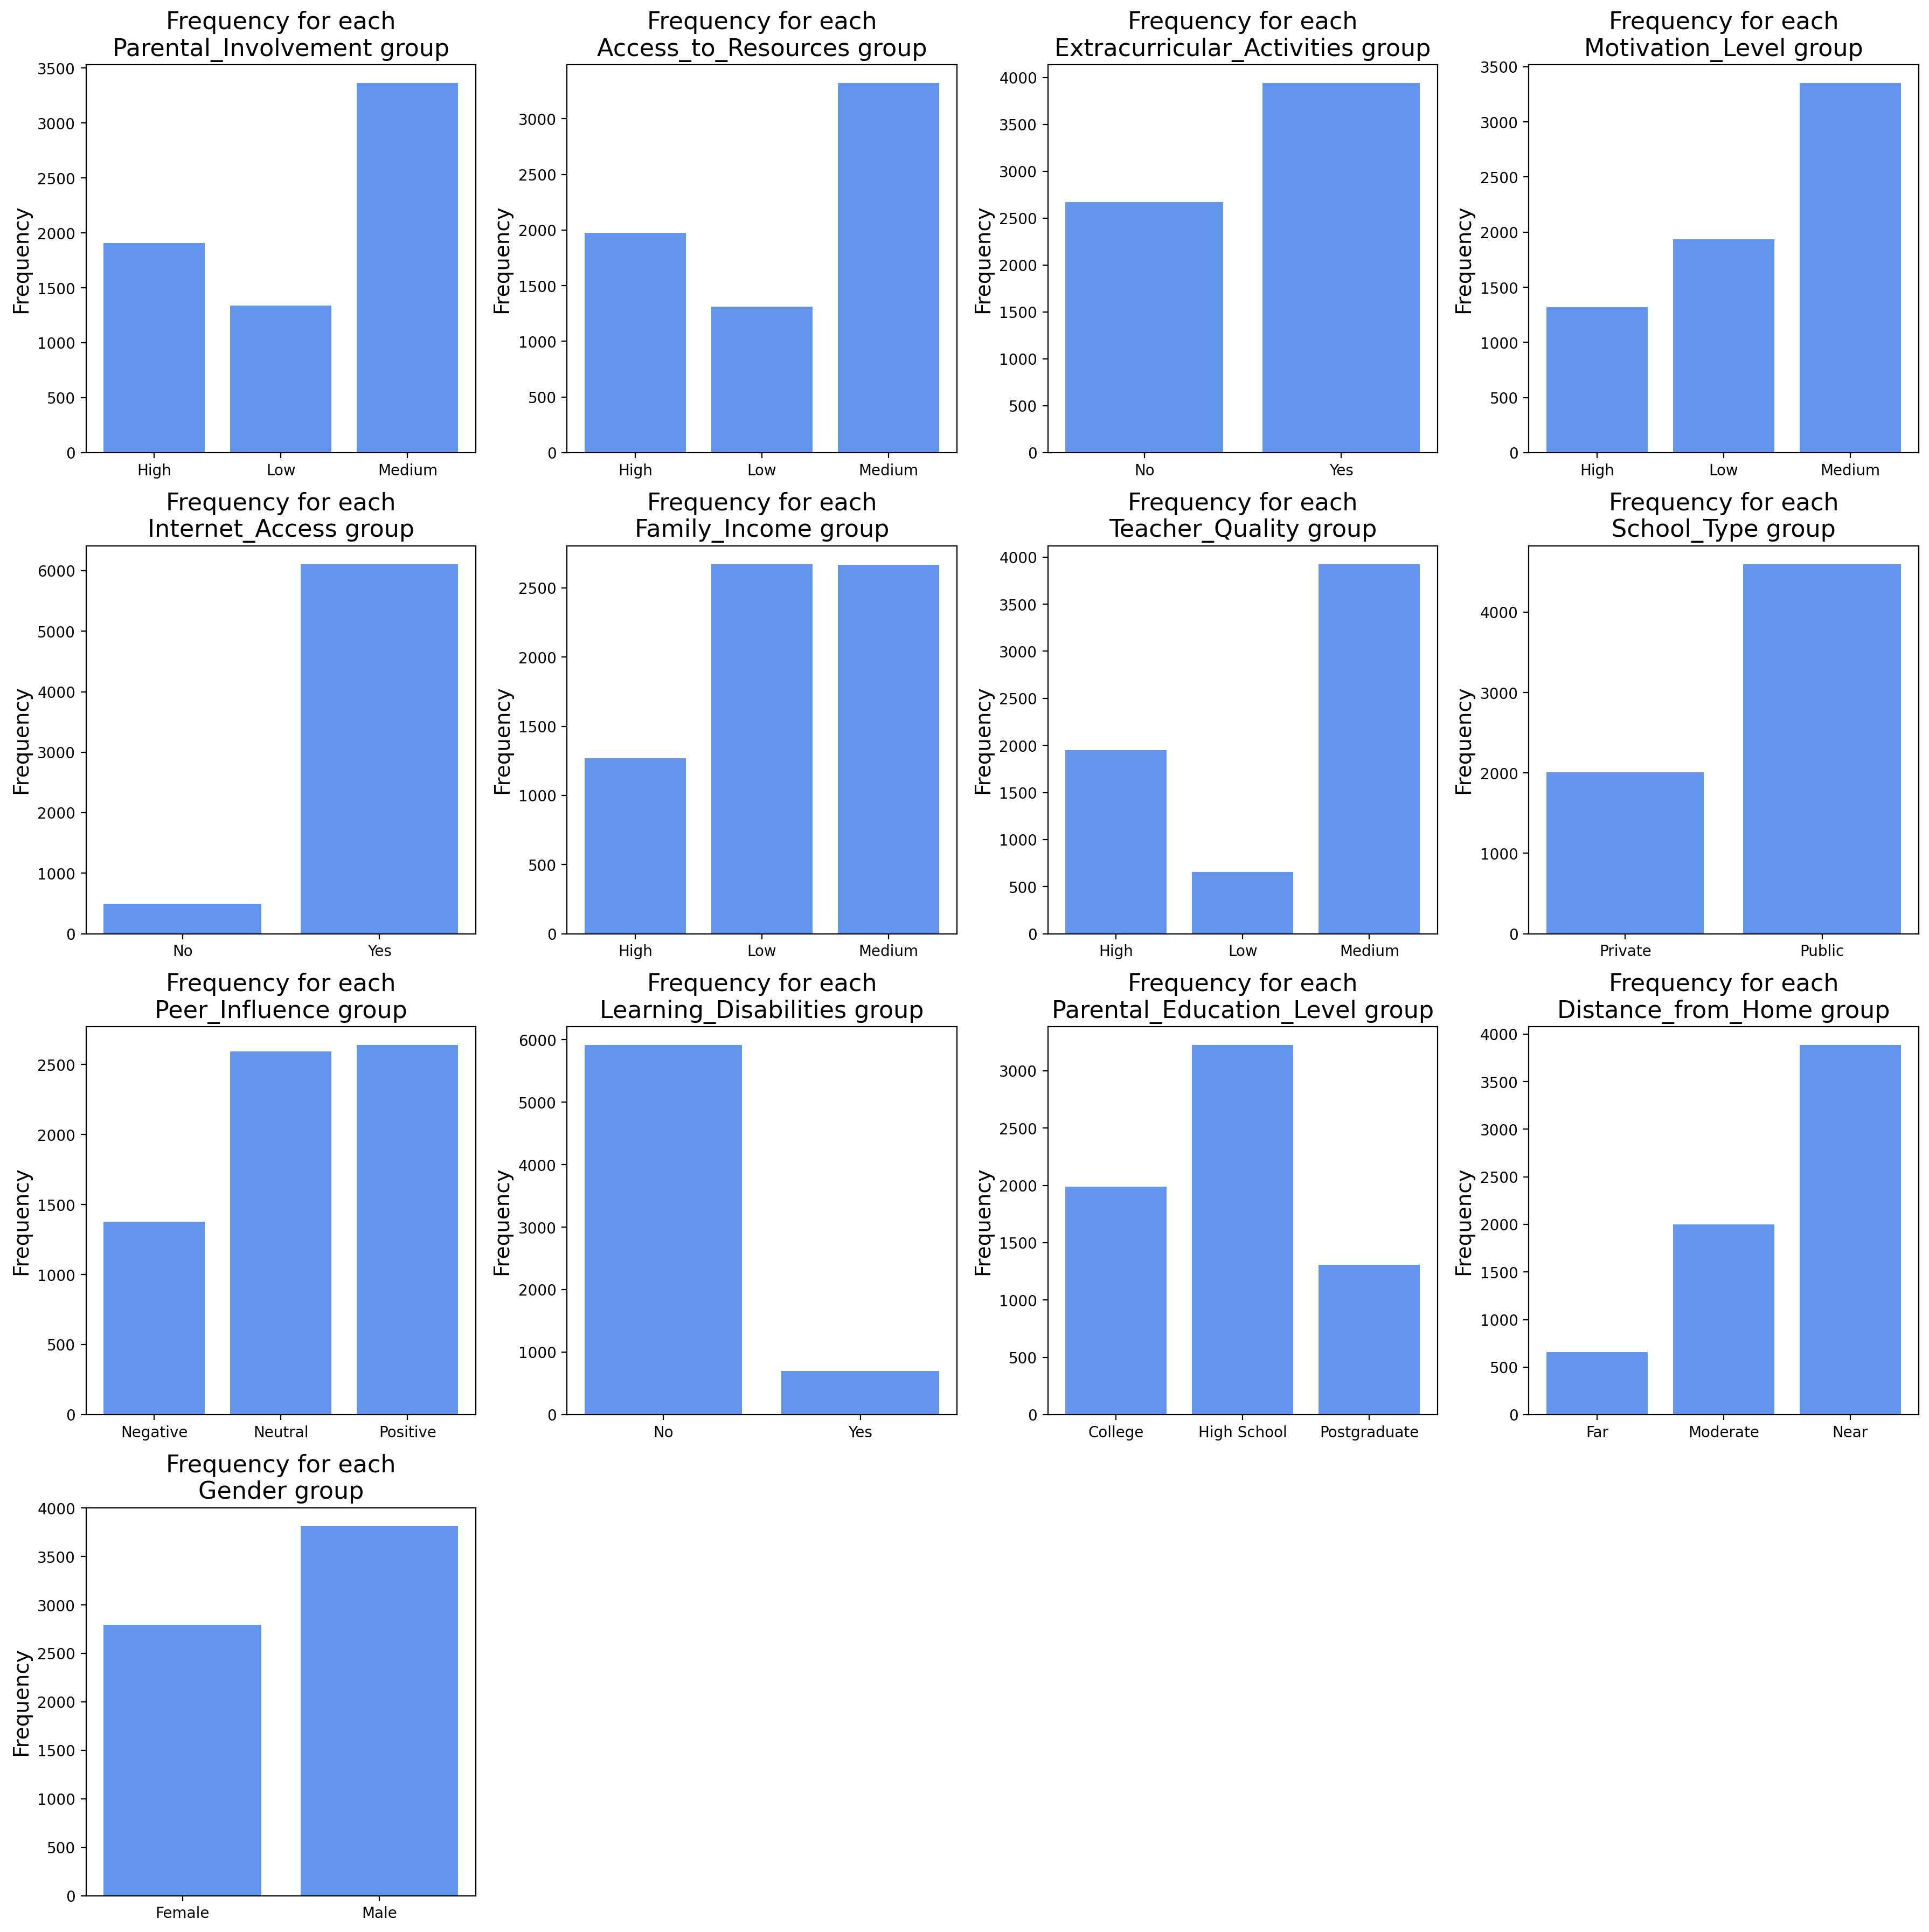
\includegraphics[width=0.9\columnwidth]{1-barplots.png}
  \caption{Plotting the frequency of each category for our categorical variables.}
  \label{1:barplots}
\end{figure*}

\newpage
\renewcommand{\tablename}{Supplementary Table}
\setcounter{table}{0}

\begin{table*}[ht]
  \centering
  \begin{tabular}{|c|c|c|c|}
      \hline
      \textbf{Parental Involvement/Access to Resources} & \textbf{High} & \textbf{Low} & \textbf{Medium} \\ \hline
      High   & 568  & 413  & 927  \\ \hline
      Low    & 414  & 231  & 692  \\ \hline
      Medium & 993  & 669  & 1700 \\ \hline
  \end{tabular}
  \caption{Confusion table: Parental Involvement vs. Access to Resources.}
  \label{tab:confusion1}
\end{table*}

\begin{table*}[ht]
  \centering
  \begin{tabular}{|c|c|c|c|}
      \hline
      \textbf{Peer Influence/Family Income} & \textbf{High} & \textbf{Low} & \textbf{Medium} \\ \hline
      Negative & 251 & 577 & 549 \\ \hline
      Neutral  & 493 & 1038 & 1061 \\ \hline
      Positive & 525 & 1057 & 1056 \\ \hline
  \end{tabular}
  \caption{Confusion table: Family Income vs. Peer Influence.}
  \label{tab:confusion2}
\end{table*}

\begin{table*}[ht]
  \centering
  \begin{tabular}{|c|c|c|c|}
      \hline
      \textbf{Distance from home/Motivation Level} & \textbf{High} & \textbf{Low} & \textbf{Medium} \\ \hline
      Far       & 142   & 185   & 331   \\ \hline
      Moderate  & 394   & 611   & 993   \\ \hline
      Near      & 773   & 1125  & 1986  \\ \hline
  \end{tabular}
  \caption{Confusion table: Motivation Level vs. Distance from Home.}
  \label{tab:confusion3}
\end{table*}

\renewcommand{\figurename}{Supplementary Figure}
\setcounter{figure}{1}

\begin{figure*}[h]
  \centering
  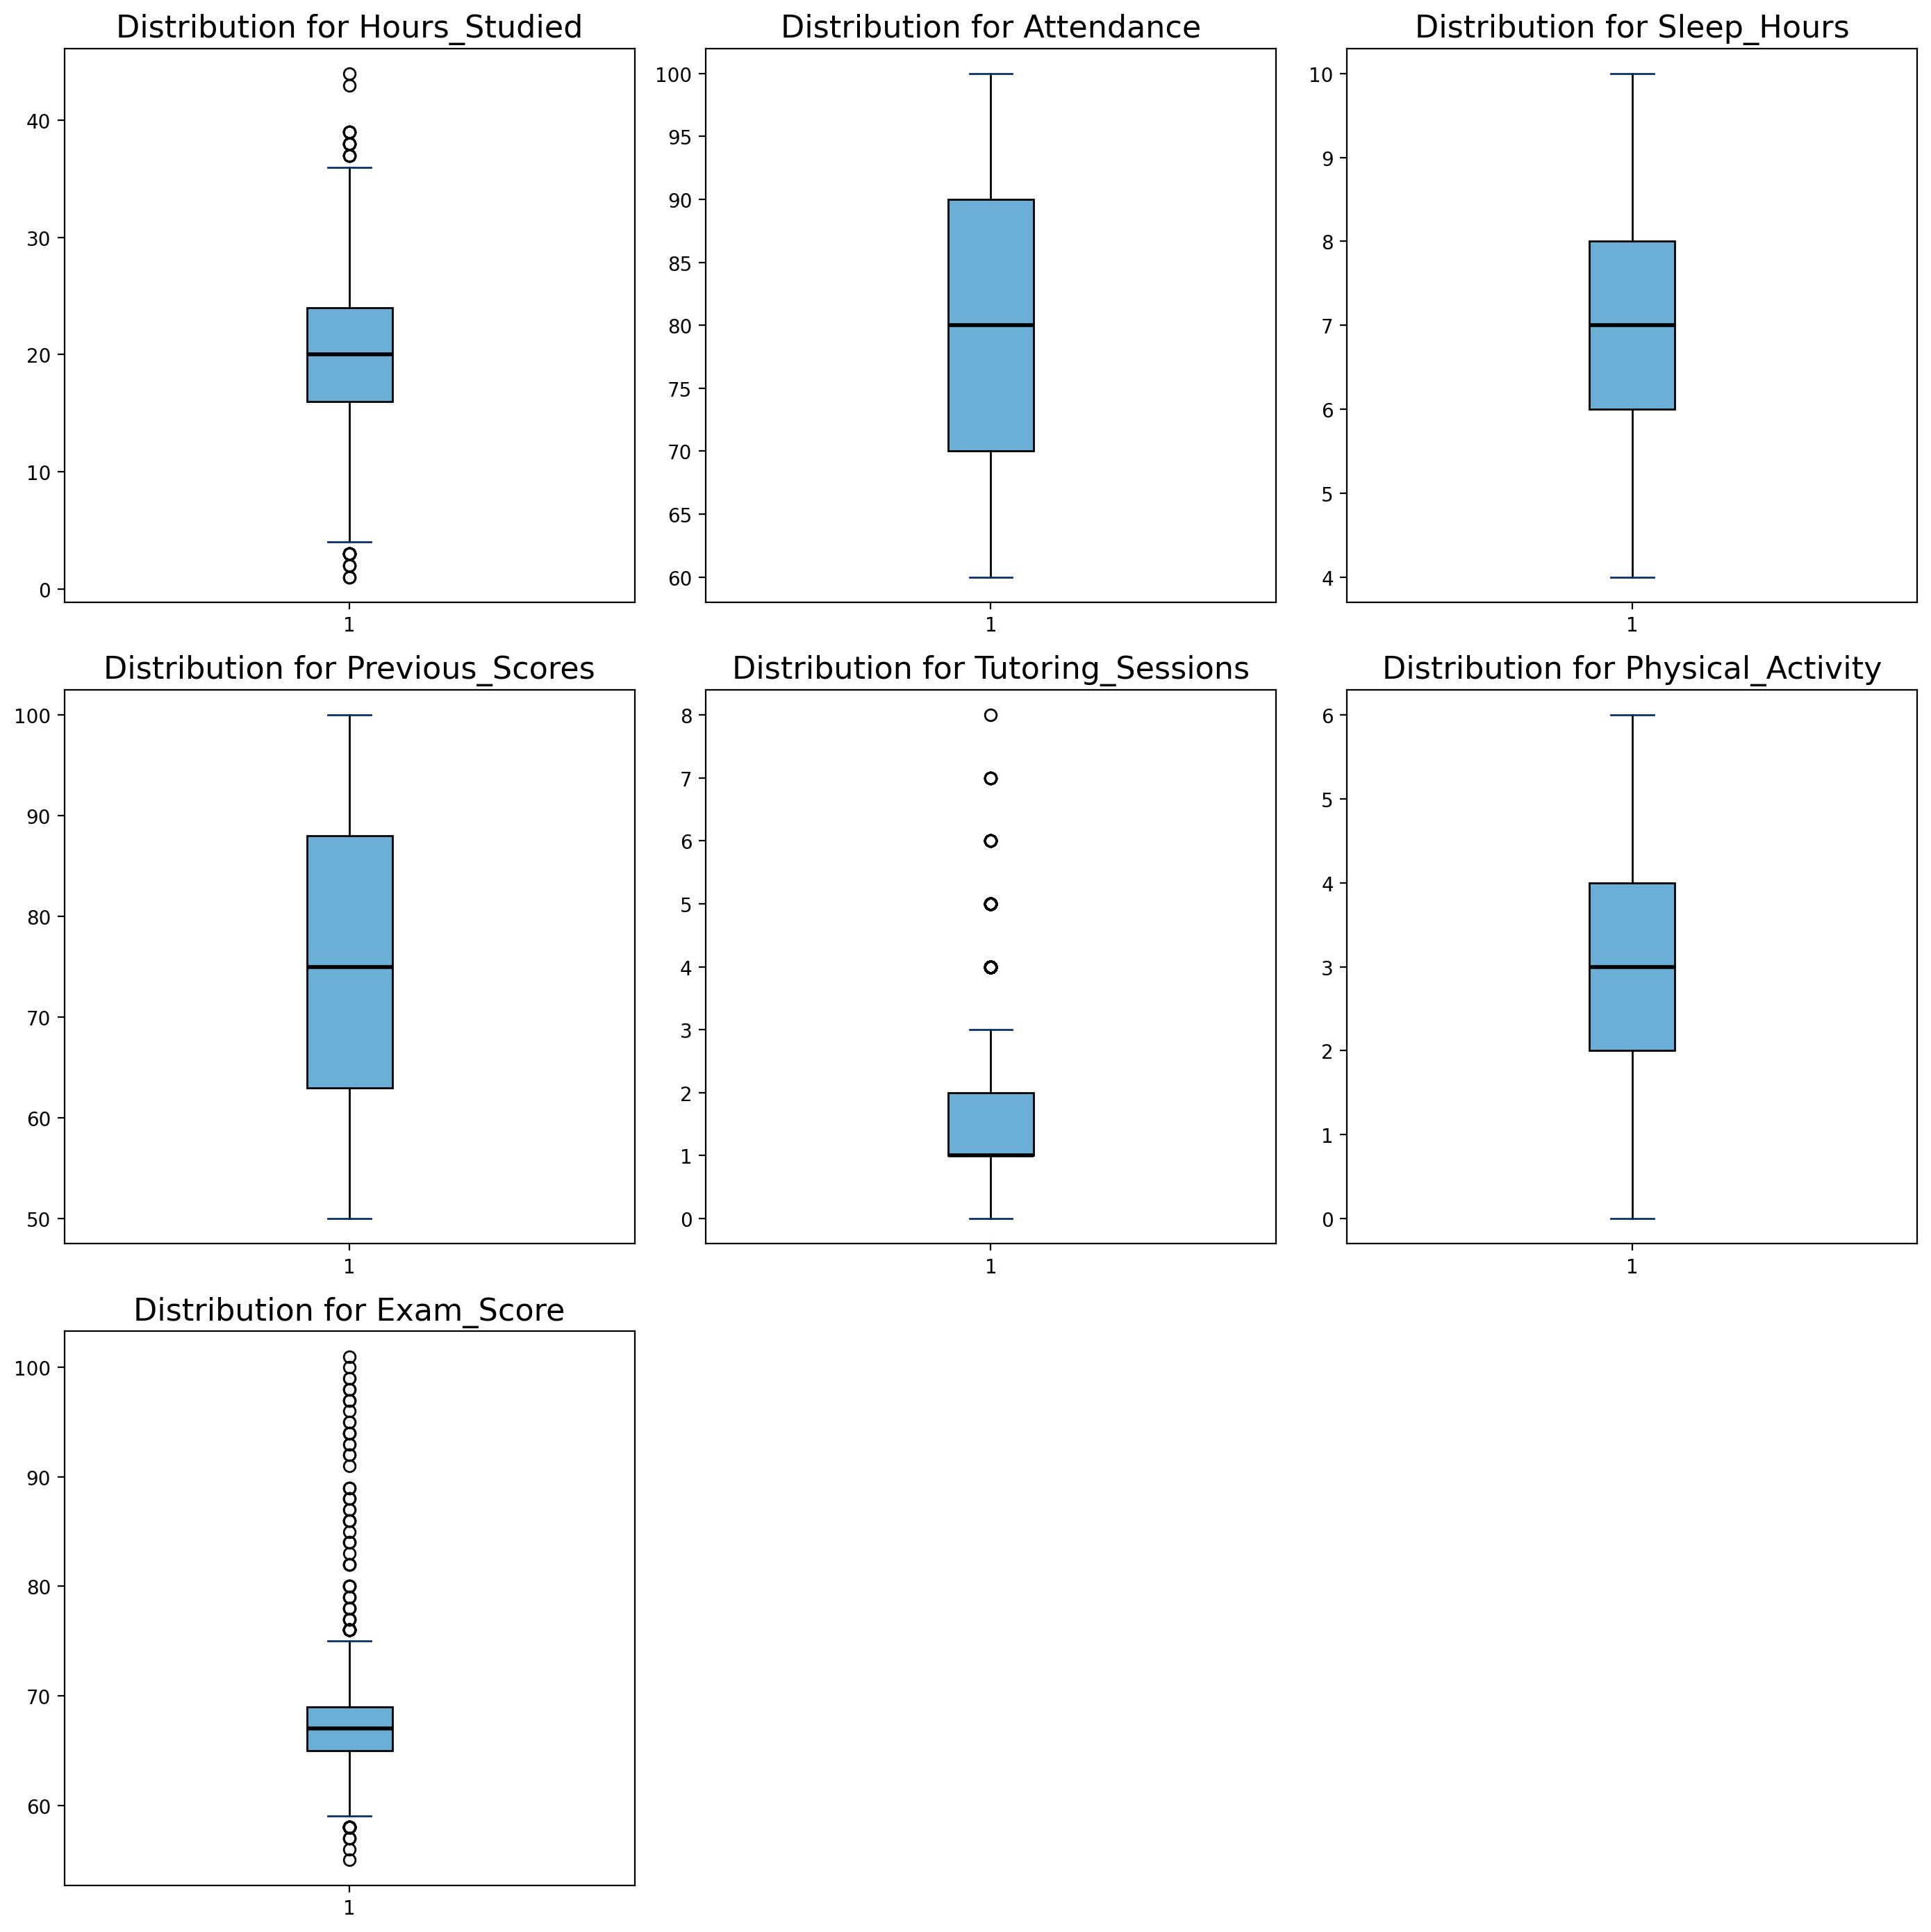
\includegraphics[width=0.9\columnwidth]{2-boxplots.png}
  \caption{Plotting the distribution of each numerical variable.}
  \label{2:boxplots}
\end{figure*}

\begin{figure*}[h]
  \centering
  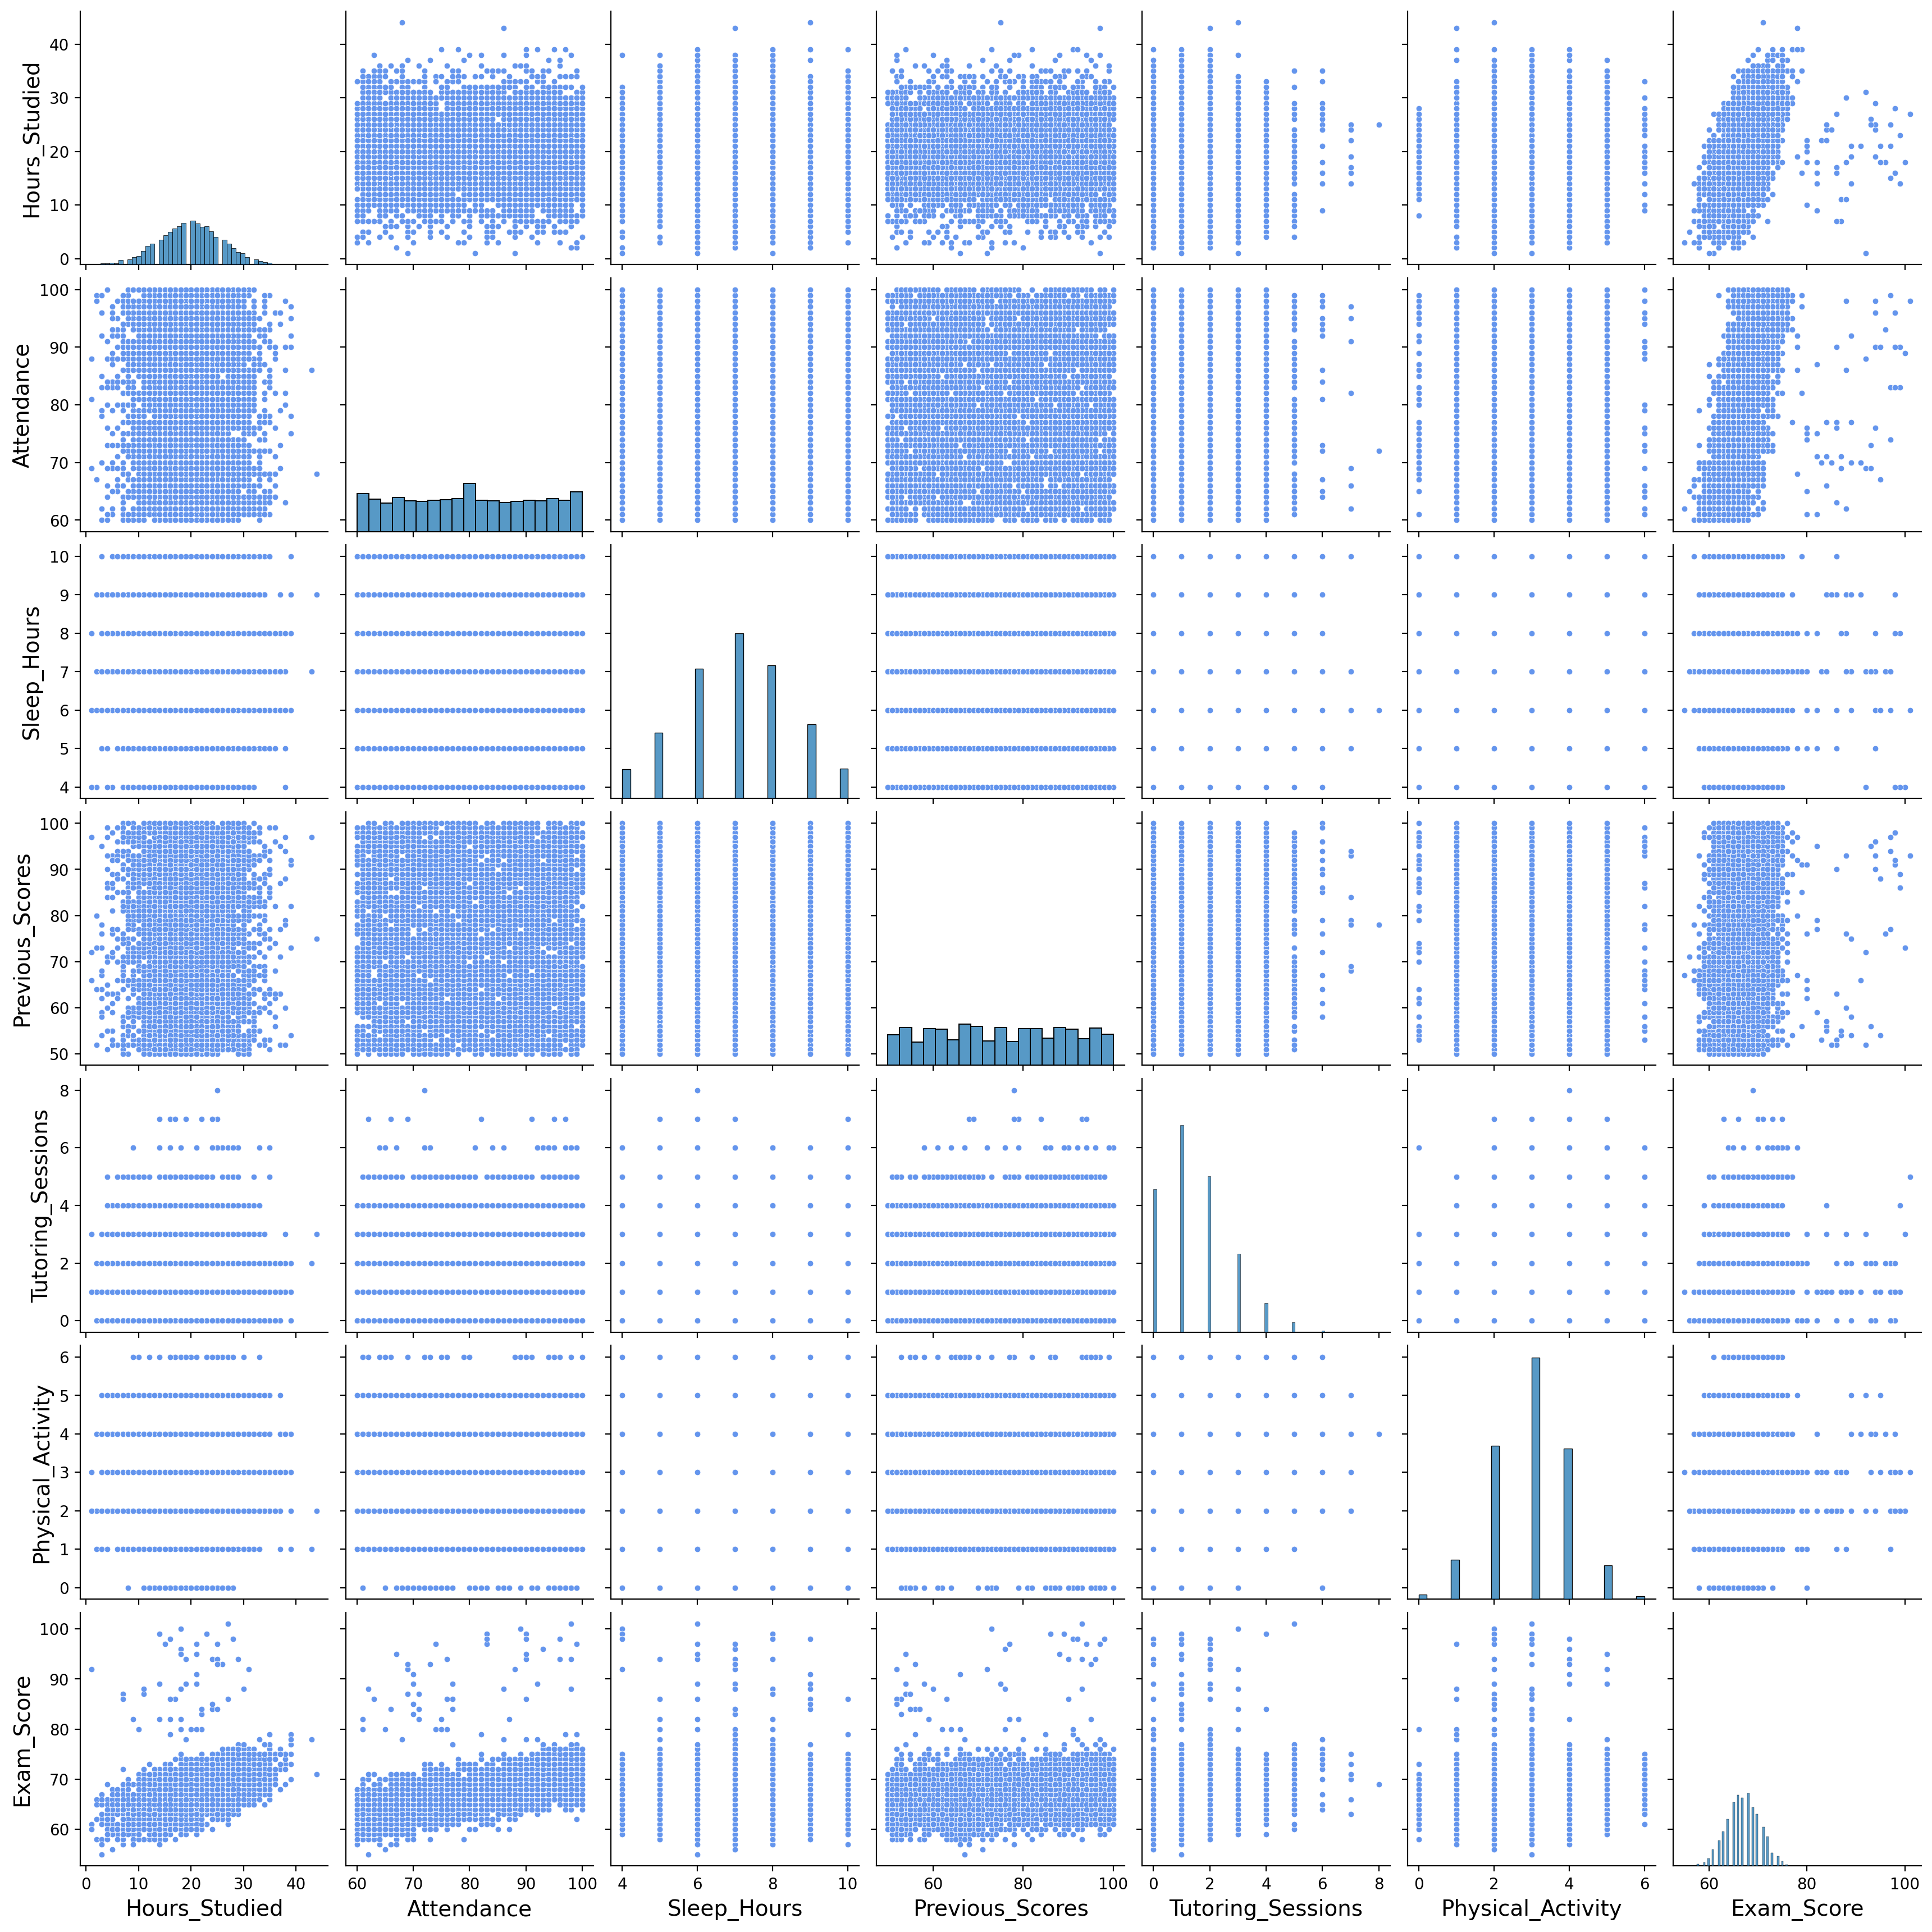
\includegraphics[width=0.9\columnwidth]{3-pairwise-plot.png}
  \caption{Numerical variable pairwise plot: Initial assessment of linear relationships between our variables.}
  \label{3:pairwise}
\end{figure*}

\renewcommand{\tablename}{Supplementary Table}
\setcounter{table}{1}

% \begin{table*}
%   \caption{Fitting an SLR model for each predictor.}
%   \label{tab:intial-model}
%   \begin{tabular}{lrrrrrrrrr}
%   \toprule
%   Predictor & Correlation & P-value & R-squared & Adj_R-squared & VIF & T-statistic & F-statistic & AIC & BIC \\
%   \midrule
%   Attendance & 0.003104 & 0.000000 & 0.336700 & 0.336596 & 1.003434 & 56.890623 & 3236.542960 & 32891.664424 & 32905.185643 \\
%   Hours_Studied & 0.003507 & 0.000000 & 0.198118 & 0.197992 & 1.002271 & 39.689943 & 1575.291562 & 34101.790605 & 34115.311825 \\
%   Previous_Scores & 0.019833 & 0.000000 & 0.030375 & 0.030223 & 1.003842 & 14.132771 & 199.735203 & 35313.278862 & 35326.800082 \\
%   Tutoring_Sessions & 0.002661 & 0.000000 & 0.024595 & 0.024442 & 1.001632 & 12.679697 & 160.774705 & 35351.180193 & 35364.701412 \\
%   Peer_Influence & 0.008092 & 0.000000 & 0.009827 & 0.009672 & 1.002203 & 7.954933 & 63.280966 & 35447.022378 & 35460.543598 \\
%   Parental_Involvement & 0.007785 & 0.000000 & 0.008843 & 0.008688 & 1.002094 & -7.542343 & 56.886934 & 35453.358706 & 35466.879926 \\
%   Access_to_Resources & 0.000353 & 0.000000 & 0.007830 & 0.007675 & 1.003961 & -7.093709 & 50.320703 & 35459.872237 & 35473.393457 \\
%   Distance_from_Home & -0.005317 & 0.000000 & 0.007759 & 0.007603 & 1.002023 & 7.060830 & 49.855316 & 35460.334142 & 35473.855361 \\
%   Learning_Disabilities & -0.005272 & 0.000000 & 0.007041 & 0.006885 & 1.002373 & -6.724033 & 45.212618 & 35464.943930 & 35478.465150 \\
%   Extracurricular_Activities & 0.013779 & 0.000000 & 0.003977 & 0.003821 & 1.001554 & 5.045584 & 25.457916 & 35484.595934 & 35498.117154 \\
%   Teacher_Quality & -0.010520 & 0.000002 & 0.003510 & 0.003354 & 1.001000 & -4.739229 & 22.460292 & 35487.583273 & 35501.104493 \\
%   Internet_Access & -0.000532 & 0.000044 & 0.002614 & 0.002457 & 1.002215 & 4.087563 & 16.708173 & 35493.319577 & 35506.840797 \\
%   Parental_Education_Level & 0.012913 & 0.001113 & 0.001666 & 0.001509 & 1.003001 & 3.261866 & 10.639768 & 35499.376896 & 35512.898116 \\
%   Physical_Activity & -0.011554 & 0.044613 & 0.000632 & 0.000476 & 1.005148 & 2.008678 & 4.034786 & 35505.976356 & 35519.497576 \\
%   Family_Income & 0.008112 & 0.070478 & 0.000513 & 0.000356 & 1.003256 & -1.809132 & 3.272958 & 35506.737986 & 35520.259206 \\
%   Motivation_Level & -0.012348 & 0.156195 & 0.000315 & 0.000159 & 1.002466 & -1.418154 & 2.011161 & 35507.999656 & 35521.520876 \\
%   Sleep_Hours & 0.010594 & 0.170317 & 0.000295 & 0.000138 & 1.002320 & -1.371340 & 1.880573 & 35508.130246 & 35521.651465 \\
%   School_Type & -0.012893 & 0.385499 & 0.000118 & -0.000039 & 1.002547 & -0.867869 & 0.753196 & 35509.257743 & 35522.778962 \\
%   Gender & 0.003920 & 0.693696 & 0.000024 & -0.000133 & 1.001838 & -0.393863 & 0.155128 & 35509.855956 & 35523.377176 \\
%   \bottomrule
%   \end{tabular}
%   \end{table*}

\end{document}
